\documentclass[ignorenonframetext,]{beamer}
\setbeamertemplate{caption}[numbered]
\setbeamertemplate{caption label separator}{: }
\setbeamercolor{caption name}{fg=normal text.fg}
\beamertemplatenavigationsymbolsempty
\usepackage{lmodern}
\usepackage{amssymb,amsmath}
\usepackage{ifxetex,ifluatex}
\usepackage{fixltx2e} % provides \textsubscript
\ifnum 0\ifxetex 1\fi\ifluatex 1\fi=0 % if pdftex
  \usepackage[T1]{fontenc}
  \usepackage[utf8]{inputenc}
\else % if luatex or xelatex
  \ifxetex
    \usepackage{mathspec}
  \else
    \usepackage{fontspec}
  \fi
  \defaultfontfeatures{Ligatures=TeX,Scale=MatchLowercase}
\fi
\usetheme{Madrid}
\usecolortheme{seahorse}
\usefonttheme{serif}
% use upquote if available, for straight quotes in verbatim environments
\IfFileExists{upquote.sty}{\usepackage{upquote}}{}
% use microtype if available
\IfFileExists{microtype.sty}{%
\usepackage{microtype}
\UseMicrotypeSet[protrusion]{basicmath} % disable protrusion for tt fonts
}{}
\newif\ifbibliography
\usepackage{natbib}
\bibliographystyle{plainnat}
\usepackage{longtable,booktabs}
\usepackage{caption}
% These lines are needed to make table captions work with longtable:
\makeatletter
\def\fnum@table{\tablename~\thetable}
\makeatother
\usepackage{graphicx,grffile}
\makeatletter
\def\maxwidth{\ifdim\Gin@nat@width>\linewidth\linewidth\else\Gin@nat@width\fi}
\def\maxheight{\ifdim\Gin@nat@height>\textheight0.8\textheight\else\Gin@nat@height\fi}
\makeatother
% Scale images if necessary, so that they will not overflow the page
% margins by default, and it is still possible to overwrite the defaults
% using explicit options in \includegraphics[width, height, ...]{}
\setkeys{Gin}{width=\maxwidth,height=\maxheight,keepaspectratio}

% Prevent slide breaks in the middle of a paragraph:
\widowpenalties 1 10000
\raggedbottom

\AtBeginPart{
  \let\insertpartnumber\relax
  \let\partname\relax
  \frame{\partpage}
}
\AtBeginSection{
  \ifbibliography
  \else
    \let\insertsectionnumber\relax
    \let\sectionname\relax
    \frame{\sectionpage}
  \fi
}
\AtBeginSubsection{
  \let\insertsubsectionnumber\relax
  \let\subsectionname\relax
  \frame{\subsectionpage}
}

\setlength{\emergencystretch}{3em}  % prevent overfull lines
\providecommand{\tightlist}{%
  \setlength{\itemsep}{0pt}\setlength{\parskip}{0pt}}
\setcounter{secnumdepth}{0}
\usepackage{textpos}
\usepackage{mathpazo}

\definecolor{first}{HTML}{009D7F}
\definecolor{first-text}{HTML}{F2F2F2}
\definecolor{second}{HTML}{00997D}
\definecolor{second-text}{HTML}{FDFDFD}
\definecolor{third}{HTML}{008068}
\definecolor{third-text}{HTML}{FFFFFF}
\setbeamercolor*{palette primary}{use=structure,fg=first-text,bg=first}
\setbeamercolor*{palette secondary}{use=structure,fg=second-text,bg=second}
\setbeamercolor*{palette tertiary}{use=structure,fg=third-text,bg=third}
\setbeamercolor{item projected}{fg=white,bg=third}

\addtobeamertemplate{frametitle}{}{%
\begin{textblock*}{100mm}(0.92\textwidth,-0.85cm)

\includegraphics[height=0.75cm]{LogoNMBUwhite}
\end{textblock*}}

\titlegraphic{
\includegraphics[height=1cm]{LogoNMBU}}
% \renewcommand*{\bibfont}{\scriptsize}

\makeatletter
\setbeamertemplate{footline}
{
  \leavevmode%
  \hbox{%
  \begin{beamercolorbox}[wd=.15\paperwidth,ht=2.25ex,dp=1ex,center]{author in head/foot}%
    \usebeamerfont{author in head/foot}\insertshortauthor
  \end{beamercolorbox}%
  \begin{beamercolorbox}[wd=.6\paperwidth,ht=2.25ex,dp=1ex,center]{title in head/foot}%
    \usebeamerfont{title in head/foot}\inserttitle
  \end{beamercolorbox}%
  \begin{beamercolorbox}[wd=.25\paperwidth,ht=2.25ex,dp=1ex,right]{date in head/foot}%
    \usebeamerfont{date in head/foot}\insertshortdate{}\hspace*{2em}
    \insertframenumber{} / \inserttotalframenumber\hspace*{2ex} 
  \end{beamercolorbox}}%
  \vskip0pt%
}
\makeatother

\title{A comparetive study on PCR, PLS, Envelope and BayesPLS models}
\author{Raju Rimal}
\institute{\textbf{Supervisors}\\
Solve Sæbø, Tryge Almøy\\
\&\\
\textbf{Joint work with}\\
Inge Halland, UiO}
\date{4 September 2016}

\begin{document}
\frame{\titlepage}

\begin{frame}{Overview}

\begin{itemize}
\tightlist
\item
  Background
\item
  Estimation methods under comparison
\item
  Data Simulation
\item
  Analysis, Results and Discussions
\end{itemize}

\end{frame}

\begin{frame}{Background}

\begin{itemize}[<+->]
\tightlist
\item
  PLS \textbf{Population Model} \citep{helland1990partial} which further
  discussed by \citep{naes1993relevant, helland2001some}
\item
  PLS, \emph{heavely developed}
  \citep{wold1985partial, naes1993relevant, de1993simpls}, without
  addressing the population model \citep{cook2013envelopes}
\item
  Mostly popular among chemometrician
\item
  Was not very popular among statistician which has changed and is
  nowadays considered as an essential tool for multivariate analysis
\item
  Accounting the population model, new estimation methods have been
  purposed such as \textbf{Envelope}
  \citep{cook2010envelope, cook2016algorithms} and \textbf{BayesPLS}
  \citep{helland2012near} which are \emph{closely related} to PLS
\item
  \citet{cook2013envelopes} said that PLS is fundamentally an envelope
  in the population model
\end{itemize}

\end{frame}

\begin{frame}[fragile]{Background}

\begin{itemize}[<+->]
\tightlist
\item
  This study attempts to make an \emph{emperial comparison} among PCR,
  PLS, Envelope and BayesPLS model on the basis of their
  \textbf{prediction ability}
\item
  Using \texttt{simrel} \citep{saebo2015simrel} R-package, data with
  diverse nature are simulated.
\item
  \texttt{simrel} allows to have control over latent structure (relevant
  component) of the data, fine analysis of strength and weakness of a
  models is possible
\end{itemize}

\end{frame}

\begin{frame}{Statistical Model}

The common ground of all the methods is to best describe (fit) the
multivariate linear model below,

\begin{equation}
\boldsymbol{y} = \boldsymbol{X}\boldsymbol{\beta} + \boldsymbol{\epsilon}
\label{eq:model}
\end{equation}

where,

\begin{longtable}[]{@{}lll@{}}
\toprule
\(\boldsymbol{y}\) & : & Response\tabularnewline
\(\boldsymbol{X}\) & : & Matrix of \(p\) predictor
variable\tabularnewline
\(\boldsymbol{\beta}\) & : & Regression Coefficients\tabularnewline
\(\boldsymbol{\epsilon}\) & : & Error
\(\epsilon \sim \text{NID}(0, \sigma^2)\)\tabularnewline
\bottomrule
\end{longtable}

Here, both \(\boldsymbol{y}\) and \(\boldsymbol{X}\) are considered to
be centered.

\end{frame}

\begin{frame}{Statistical Model}

All the models under this study consider a \textbf{subspace of predictor
variables that is relevant for response}. They differ in the ways of
finding the subspace and corresponding model estimates. The true
estimates can also be written as,

\[
\begin{aligned}
\boldsymbol{\beta} &= \Sigma_{XX}^{-1}\sigma_{Xy} = \sum_{j=1}^p \frac{1}{\alpha_j}\boldsymbol{e}_j\boldsymbol{e}_j^t\sigma_{Xy}
= \sum_{j=1}^p\gamma_j\boldsymbol{e}_j\\
\end{aligned}
\]

where,

\begin{longtable}[]{@{}ll@{}}
\toprule
\(\gamma_j\) & :
\(\frac{\boldsymbol{e}_j^t\sigma_{Xy}}{\lambda_j}\)\tabularnewline
\(\boldsymbol{e}_j\) & : Eigenvector of \(\Sigma_{xx}\)\tabularnewline
\(\lambda_j\) & : Eigenvalue of \(\Sigma_{xx}\)\tabularnewline
\(\sigma_{Xy}\) & : Covariance between \(y\) and \(X\)\tabularnewline
\bottomrule
\end{longtable}

So, True regression estimates are the space spanned by the eigenvectors
of population covariance matrix \(\Sigma_{xx}\).

\end{frame}

\begin{frame}{Comparison of Methods}

\begin{longtable}[]{@{}ll@{}}
\toprule
\begin{minipage}[b]{0.53\columnwidth}\raggedright\strut
PCR
\strut\end{minipage} &
\begin{minipage}[b]{0.41\columnwidth}\raggedright\strut
PLS
\strut\end{minipage}\tabularnewline
\midrule
\endhead
\begin{minipage}[t]{0.53\columnwidth}\raggedright\strut
* Regression of response on latent space of predictor
\strut\end{minipage} &
\begin{minipage}[t]{0.41\columnwidth}\raggedright\strut
* Estimation through Iterative algorithm
\strut\end{minipage}\tabularnewline
\begin{minipage}[t]{0.53\columnwidth}\raggedright\strut
* No strict assumption
\strut\end{minipage} &
\begin{minipage}[t]{0.41\columnwidth}\raggedright\strut
* No strict assumption
\strut\end{minipage}\tabularnewline
\bottomrule
\end{longtable}

\pause

\begin{longtable}[]{@{}ll@{}}
\toprule
\begin{minipage}[b]{0.45\columnwidth}\raggedright\strut
Envelope (MLE)
\strut\end{minipage} &
\begin{minipage}[b]{0.49\columnwidth}\raggedright\strut
Bayes
\strut\end{minipage}\tabularnewline
\midrule
\endhead
\begin{minipage}[t]{0.45\columnwidth}\raggedright\strut
* Estimation using Maximum Likelihood
\strut\end{minipage} &
\begin{minipage}[t]{0.49\columnwidth}\raggedright\strut
* Estimation through MCMC approach with rotation of relevant space
\strut\end{minipage}\tabularnewline
\begin{minipage}[t]{0.45\columnwidth}\raggedright\strut
* Can not be used when predictor is larger than observations
\strut\end{minipage} &
\begin{minipage}[t]{0.49\columnwidth}\raggedright\strut
* Heavy Computation when \(p\) is large
\strut\end{minipage}\tabularnewline
\bottomrule
\end{longtable}

\end{frame}

\begin{frame}[fragile]{Data Simulation}

Models are analysed under diverse nature of data. Data are simulated
using \texttt{simrel} package (R). In this study, I have included
following four design;

\begin{longtable}[]{@{}rrllr@{}}
\toprule
n & p & R2 & relpos & gamma\tabularnewline
\midrule
\endhead
50 & 15 & 0.5 & 1, 2 & 0.5\tabularnewline
50 & 40 & 0.5 & 1, 2 & 0.5\tabularnewline
50 & 15 & 0.9 & 2, 3 & 0.9\tabularnewline
50 & 40 & 0.9 & 2, 3 & 0.9\tabularnewline
\bottomrule
\end{longtable}

\begin{longtable}[]{@{}lll@{}}
\toprule
\texttt{n} & : & Number of observations\tabularnewline
\texttt{p} & : & Number of variables\tabularnewline
\texttt{R2} & : & Variation explained by the model\tabularnewline
\texttt{relpos} & : & Position of relevant components\tabularnewline
\texttt{gamma} & : & Reduction factor of eigenvalue of
\(X\)\tabularnewline
\bottomrule
\end{longtable}

For each of these design, 5000 test samples are simulated.

\end{frame}

\begin{frame}{Relevant Position and Eigenvalues}

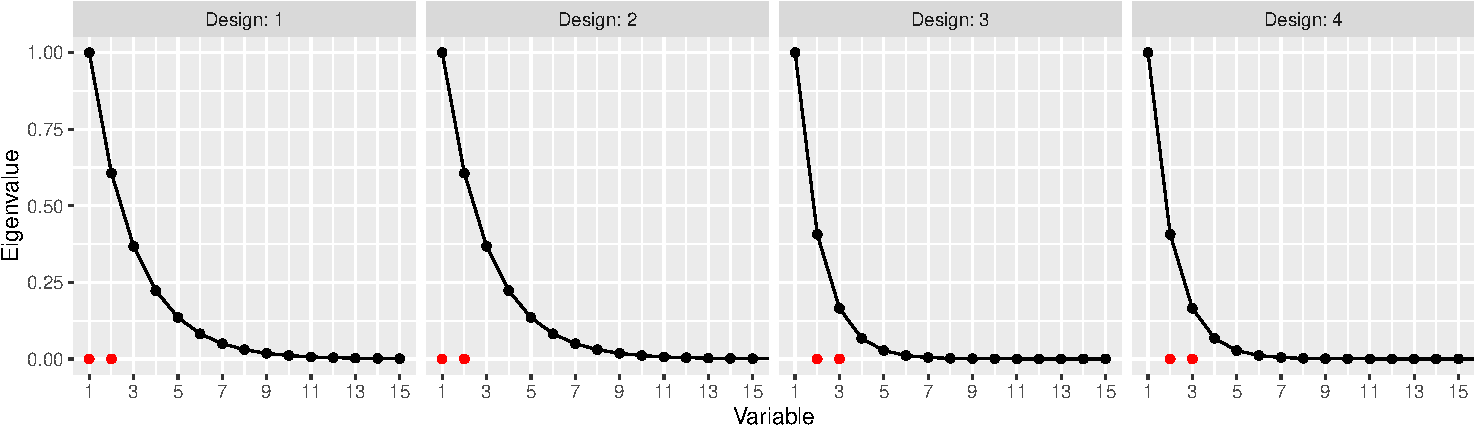
\includegraphics{Main_files/figure-beamer/unnamed-chunk-4-1.pdf}

\begin{itemize}
\tightlist
\item
  When Relevant components are at the position of high eigenvalues, the
  situation is easier to model
\item
  When Relevant components are at the position of low eigenvalues, for
  example 5, 10, then the most variation present in \(X\) are not
  relevant for \(Y\) and this will become a very difficult situation.
\end{itemize}

\end{frame}

\begin{frame}{Model assessment}

Models are compared on the basis of their prediction ability by
measuring \emph{test} and \emph{training} \textbf{Mean Square Error of
Prediction (\emph{MSEP})}. Mean prediction error is calculated as,

\[
\begin{aligned}
\left(\text{Prediction Error}\right)_\text{training} &= \frac{1}{n}\sum_{i = 1}^n\left({\boldsymbol{y}_i - \hat{\boldsymbol{y}}_i}\right)^2 = \frac{1}{n}\sum_{i = 1}^n\left({\boldsymbol{y}_i - \left(\hat{\boldsymbol{\beta}}_0 + \hat{\boldsymbol{\beta}}\boldsymbol{X}_i\right)}\right)^2 \\
\left(\text{Prediction Error}\right)_\text{test} &= \frac{1}{n}\sum_{i = 1}^\text{ntest}\left({\boldsymbol{y}_{i\left(\text{test}\right)} - \hat{\boldsymbol{y}}_{i\left(\text{test}\right)}}\right)^2 \\ &= \frac{1}{n}\sum_{i = 1}^\text{ntest}\left({\boldsymbol{y}_{i\left(\text{test}\right)} - \left(\hat{\boldsymbol{\beta}}_0 + \hat{\boldsymbol{\beta}}\boldsymbol{X}_{i\left(\text{test}\right)}\right)}\right)^2
\end{aligned}
\]

\end{frame}

\begin{frame}{Analysis Results}

\begin{center}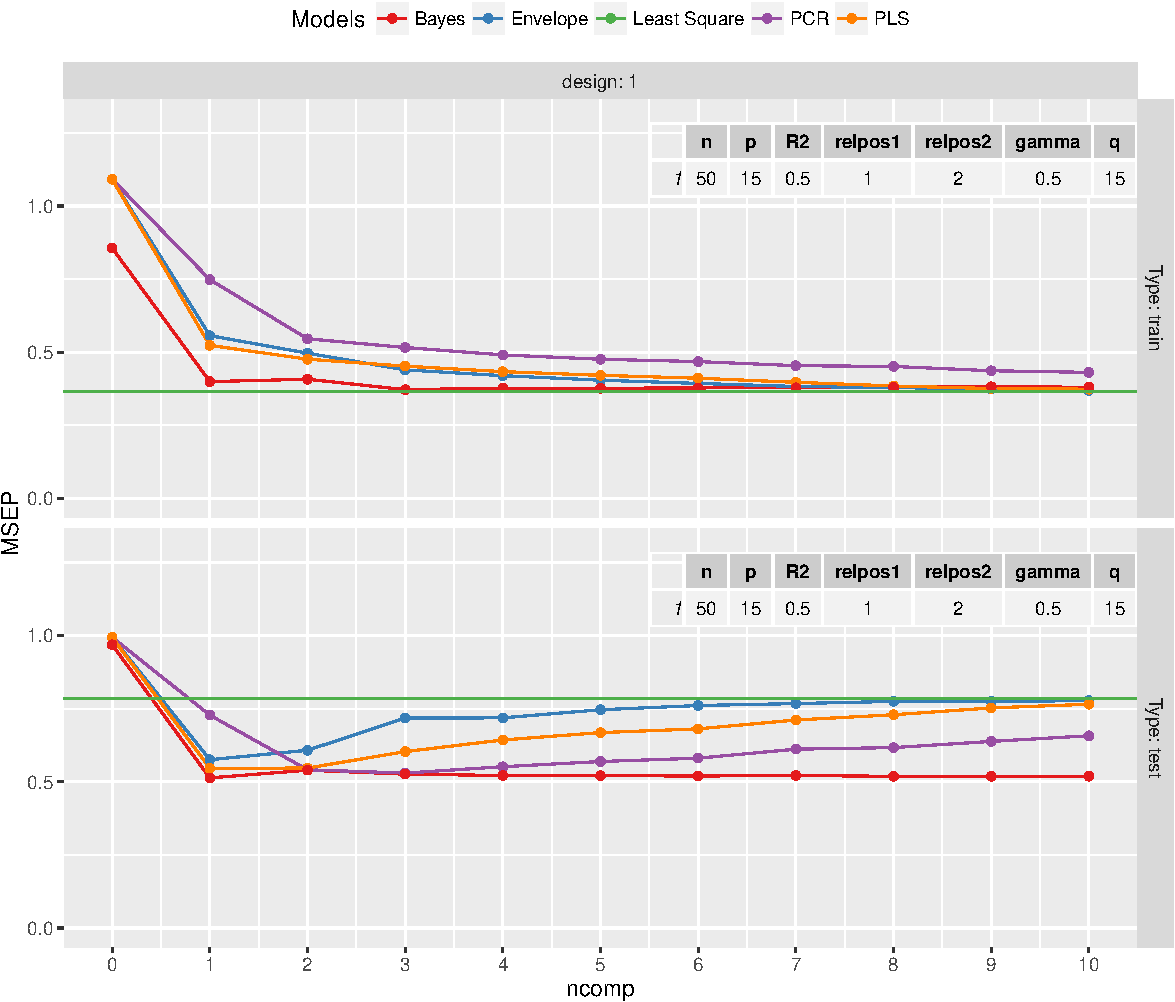
\includegraphics{Main_files/figure-beamer/unnamed-chunk-6-1} \end{center}

\end{frame}

\begin{frame}{Analysis Results}

\begin{center}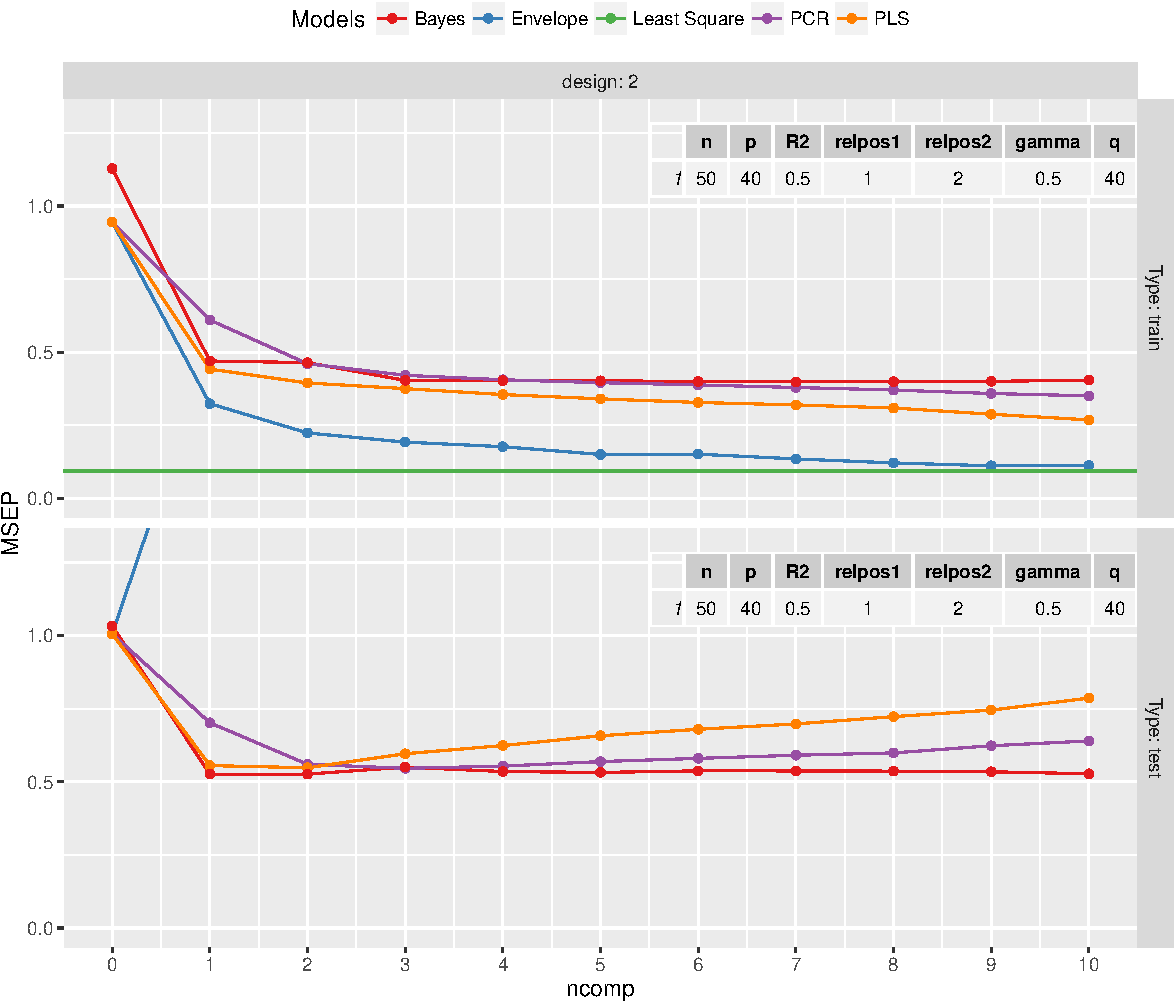
\includegraphics{Main_files/figure-beamer/unnamed-chunk-7-1} \end{center}

\end{frame}

\begin{frame}{Analysis Results}

\begin{center}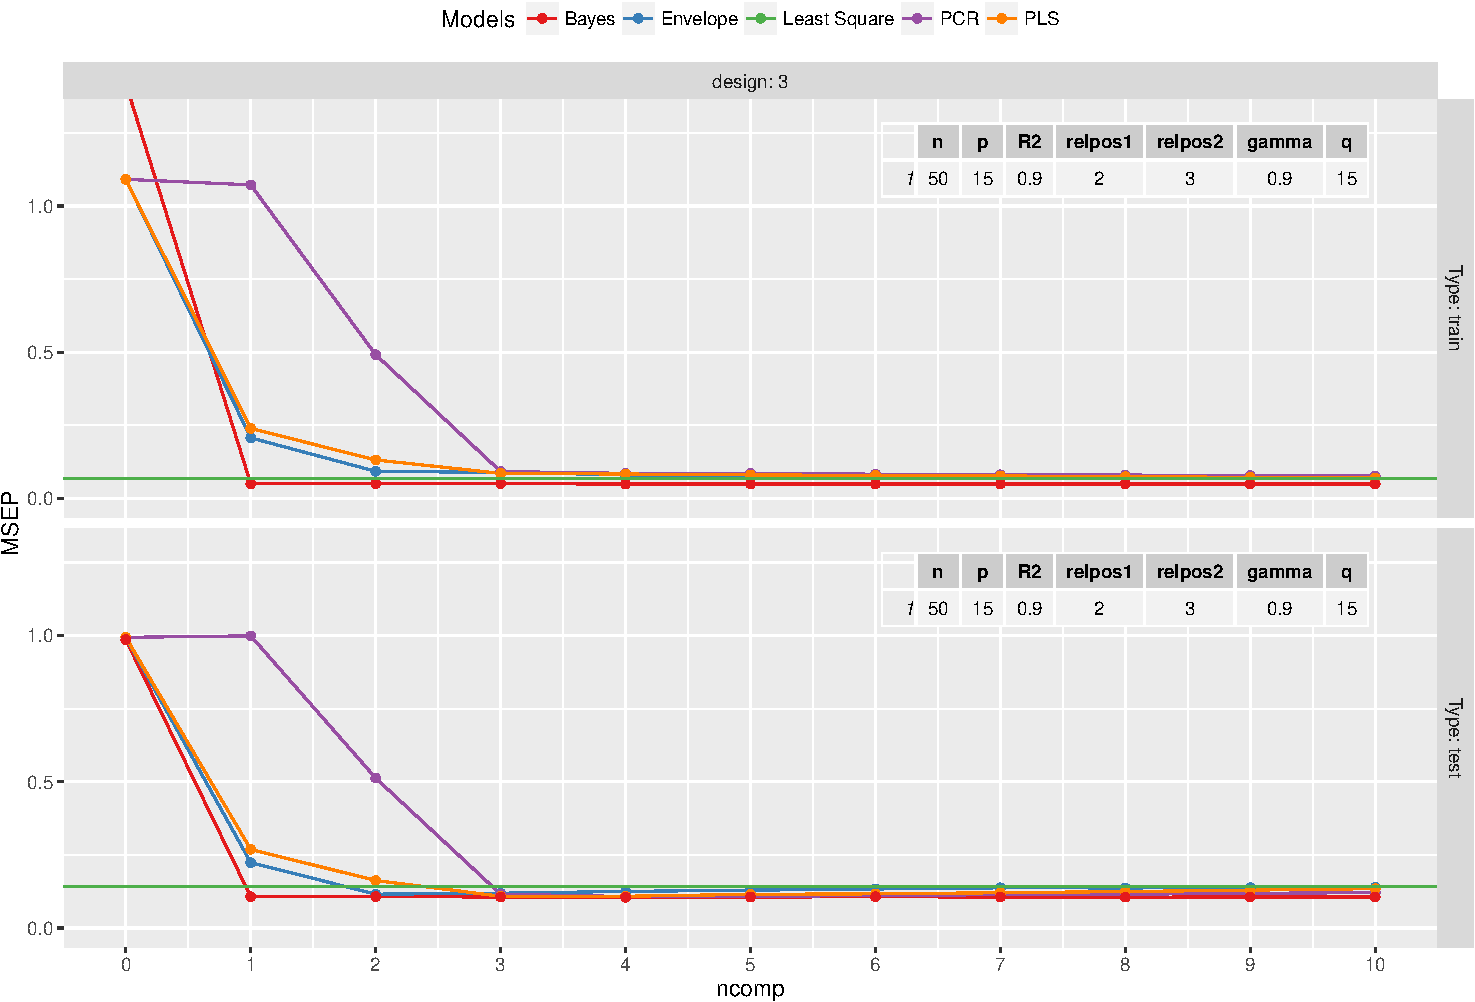
\includegraphics{Main_files/figure-beamer/unnamed-chunk-8-1} \end{center}

\end{frame}

\begin{frame}{Analysis Results}

\begin{center}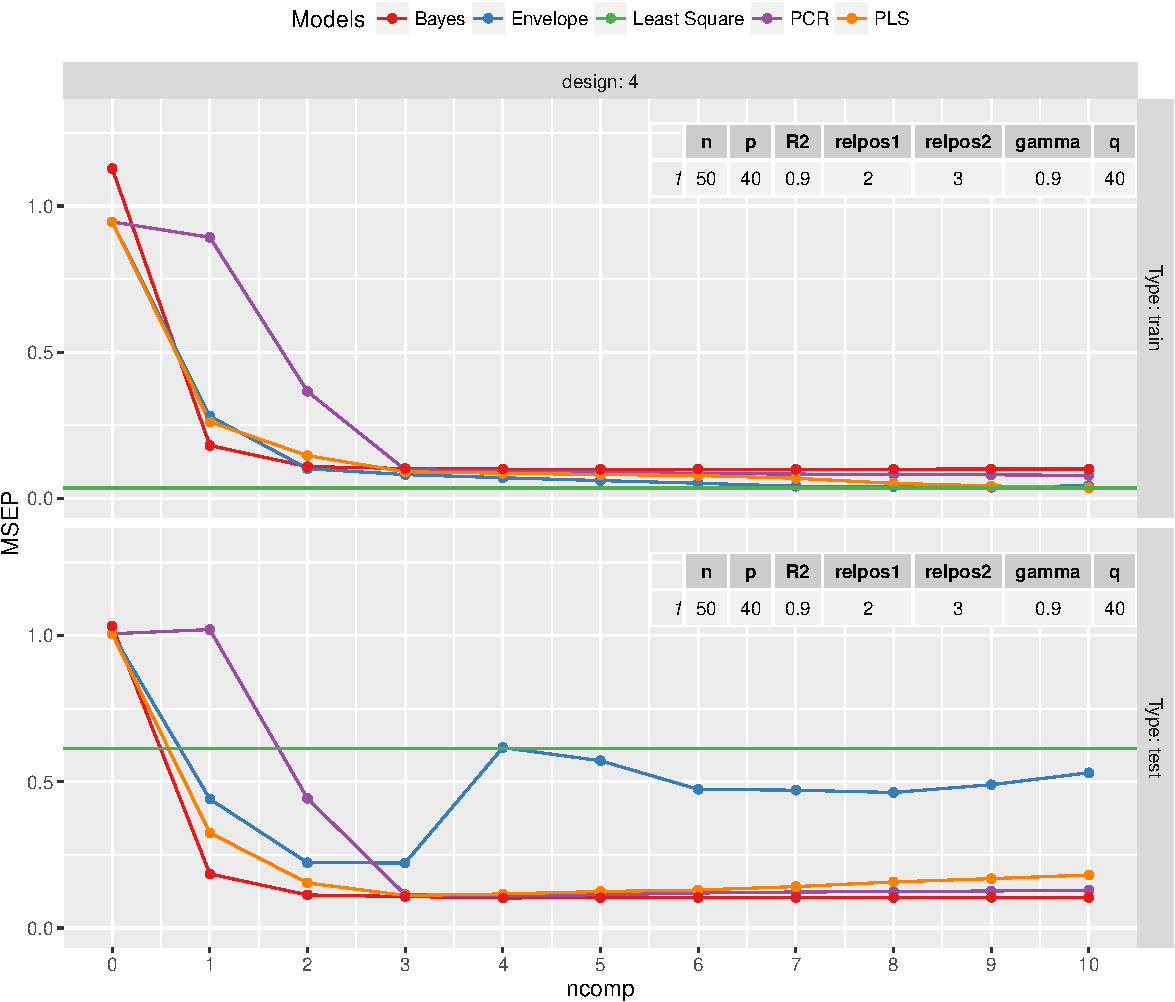
\includegraphics{Main_files/figure-beamer/unnamed-chunk-9-1} \end{center}

\end{frame}

\begin{frame}{Analysis Results}

\begin{center}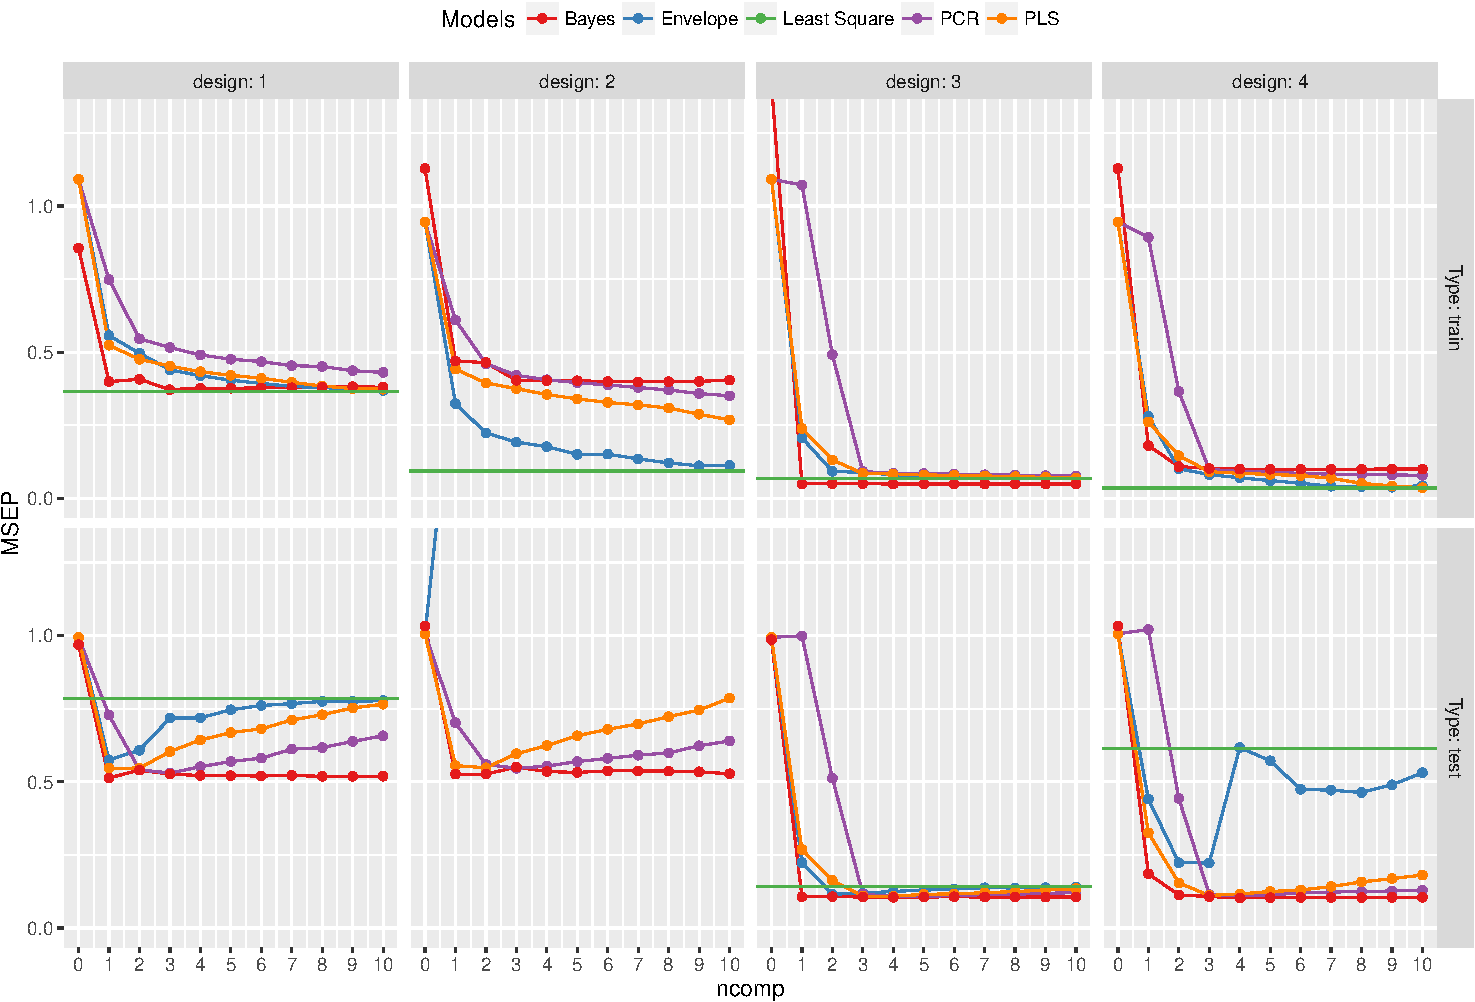
\includegraphics{Main_files/figure-beamer/unnamed-chunk-10-1} \end{center}

\end{frame}

\begin{frame}{Conclusion}

\begin{itemize}[<+->]
\tightlist
\item
  New methods -- Envelope and Bayes, as they claim, are performing
  better than algorithmic approach of PLS
\item
  However, the performance of MLE approach of Envelope is not
  satisfactory when number of variable is large
\item
  In the case of Bayes PLS, the prediction error does not raises
  noticably (test prediction) after capturing enough information with
  few components
\item
  This suggests that it is able to find the direction of maximum
  variation after successive rotations of predictor subspace
\item
  The computation regarding BayesPLS is intensive which will not be
  fisible in case of wide dataset (very common in genomic data)
\item
  All the models are performing better than the least square solution
\end{itemize}

\end{frame}

\begin{frame}

\begin{center}
\includegraphics{ThankYou} \end{center}

\end{frame}

\section{References}\label{references}

\begin{frame}[allowframebreaks]{}
\bibliographytrue
\bibliography{references.bib}
\end{frame}

\end{document}
